\documentclass[lang=cn,11pt,a4paper,cite=authornum]{paper}

\title{Linux开发环境及应用 上机作业三:脚本程序设计 \\ 实验报告}
\author{毛子恒 \\ 2019211397}
\institute{北京邮电大学\ 计算机学院}

\date{\zhtoday}

\setmonofont{Consolas}

% 本文档命令
\nocite{*}

\begin{document}

\maketitle

\part{生成TCP活动状况报告}

\section{实验内容}

\mintinline{shell}{netstat --statistics}命令可以列出tcp等协议的统计信息。编写shell脚本程序,每隔1分钟生成1行信息:当前时间;这一分钟内TCP发送了多少报文;接收了多少报文;收发报文总数;行尾给出符号+或-或空格(+表示这分钟收发报文数比上分钟多10包以上,差别在10包或以内用空格,否则用符号-)。

\section{实验步骤}

\paragraph{观察netstat命令输出}

\mintinline{shell}{netstat}命令输出的TCP部分如\figref{fig:p1}所示。 

\begin{figure}[!htb]
    \centering
    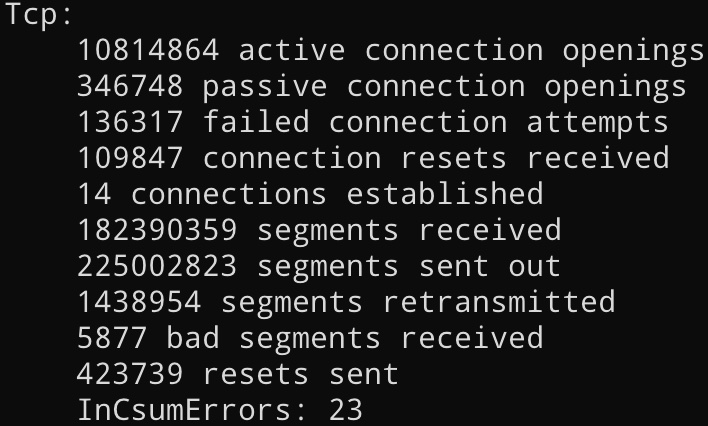
\includegraphics[width=0.5\textwidth]{./images/l3-p1.jpg}
    \caption{netstat命令的输出\label{fig:p1}}
\end{figure}

我们只需要获取segments received和segments sent out这两行,并且和上次结果进行一些算术运算即可。另外需要记录一下每两次之间的差值,与上次的差值进行比较以决定输出行末的符号。

\paragraph{编写程序}

\begin{code}
\begin{minted}{shell}
#!/bin/bash

command_res=`netstat --statistics`
last_recv=`expr "$command_res" : '^.* \([0-9][0-9]*\) segments received'`
last_sent=`expr "$command_res" : '^.* \([0-9][0-9]*\) segments sent out'`
last_total=0
#echo "$last_recv" "$last_sent"

first_min=1

while true
do
    sleep 60
    command_res=`netstat --statistics`
    recv=`expr "$command_res" : '^.* \([0-9][0-9]*\) segments received'`
    sent=`expr "$command_res" : '^.* \([0-9][0-9]*\) segments sent out'`
    date=`date "+%Y-%m-%d %H:%M"`
    
    recv_delta=`expr $recv - $last_recv`
    sent_delta=`expr $sent - $last_sent`
    total=`expr $recv_delta + $sent_delta`
    total_delta=`expr $total - $last_total`

    if [ $first_min = 1 ]
    then
        echo $date $sent_delta $recv_delta $total
        first_min=0
    else
        if [ $total_delta -ge 10 ]
        then
            echo $date $sent_delta $recv_delta $total +
        elif [ $total_delta -le 0 ]
        then
            echo $date $sent_delta $recv_delta $total -
        else
            echo $date $sent_delta $recv_delta $total -
        fi
    fi
    last_recv=$recv
    last_sent=$sent
    last_total=$total
done
\end{minted}
\end{code}

\paragraph{运行结果}

运行结果如\figref{fig:p2}。

\begin{figure}[!htb]
    \centering
    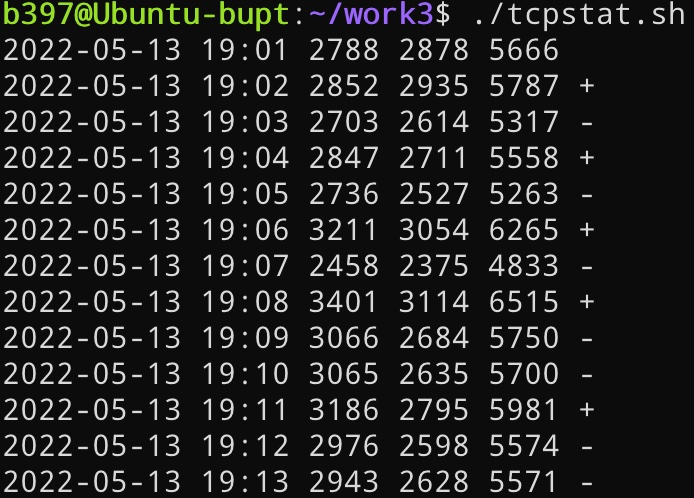
\includegraphics[width=0.5\textwidth]{./images/l3-p2.jpg}
    \caption{运行结果\label{fig:p2}}
\end{figure}

\part{下载bing图库中图片}

\section{实验内容}

访问\href{http://bing.plmeizi.com/?page=2}{http://bing.plmeizi.com/?page=2}可以看到bing图库第2页的内容,如\figref{fig:p3}所示,这个Web页有多个图片小样,小样下有中文说明信息“正在投喂幼鸟的戴胜鸟,德国”和日期信息2022-04-30,点击一下,此图片就可以在新标签页中预览。

编写脚本程序\mintinline{shell}{bing.sh},将图库中照片全部下载下来存放到本地bing目录,上面URL中page=2可以换成page=126可访问126号页面,每页有9个图,每个图的日期,中文说明信息和下载地址及文件名html文件中可提取。要求下载后的文件命名为“日期 说明.jpg”例如:“2022-04-30 正在投喂幼鸟的戴胜鸟,德国.jpg”

\begin{figure}[htbp]
    \centering
    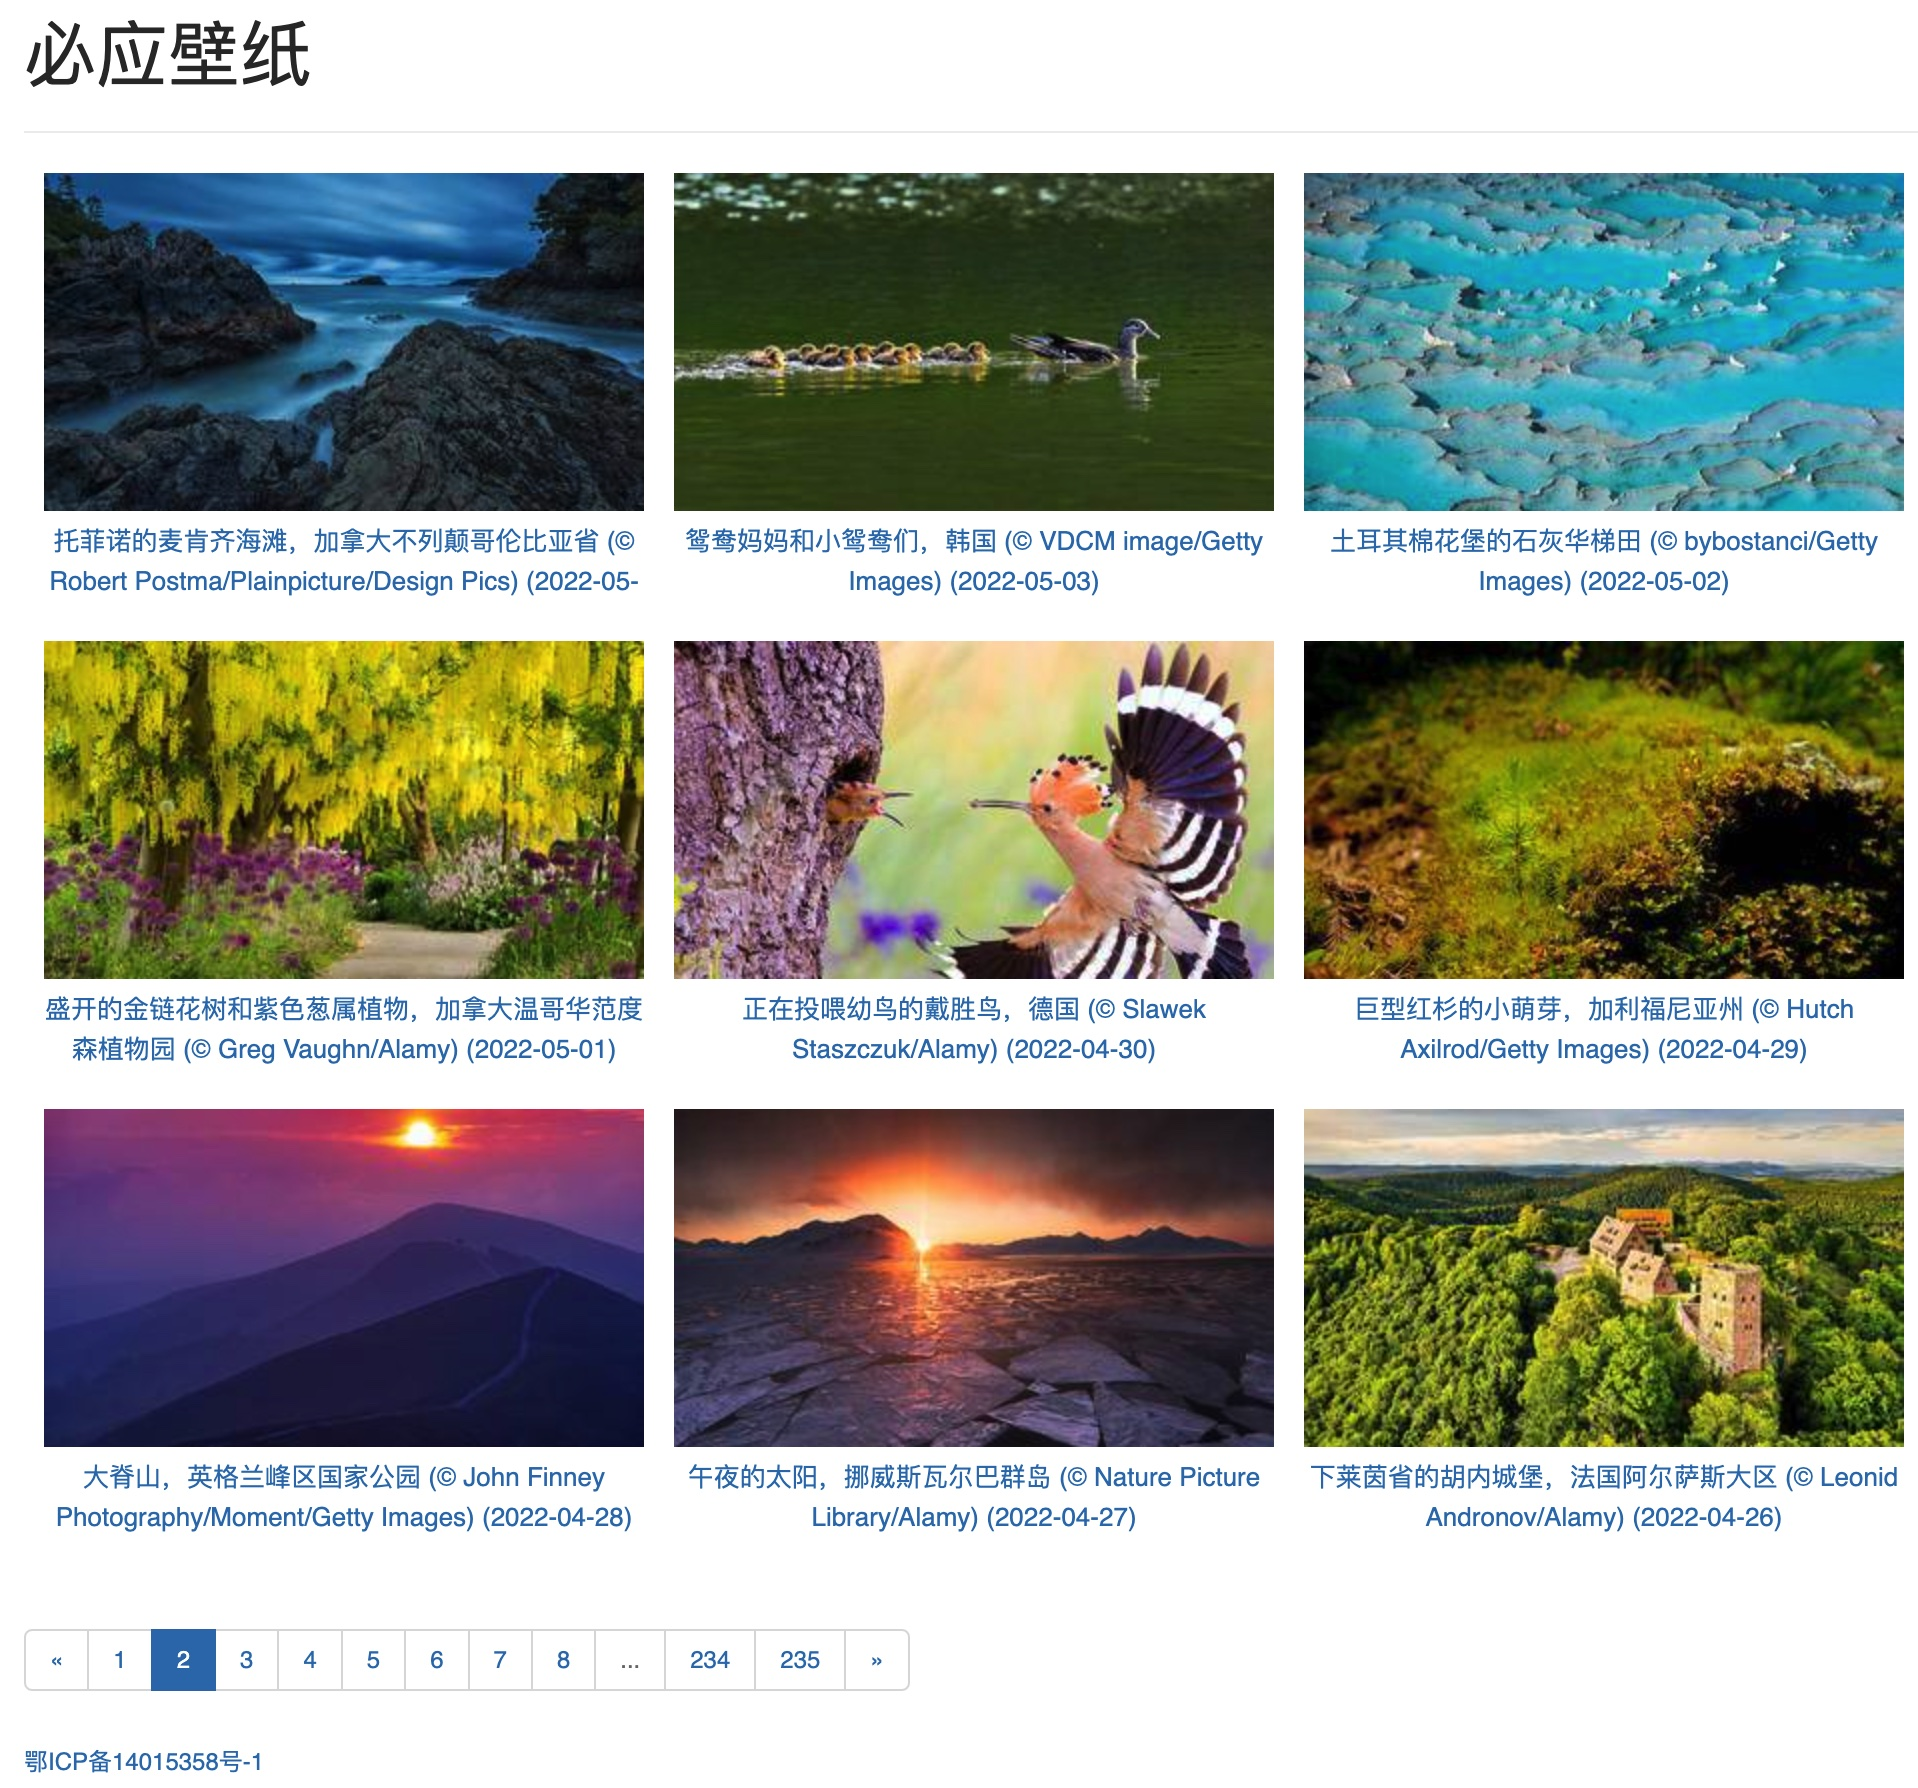
\includegraphics[width=\textwidth]{./images/l3-p3.jpg}
    \caption{Web页面\label{fig:p3}}
\end{figure}

\section{实验步骤}

\paragraph{观察Web页面源代码}

我们感兴趣的html代码如\figref{fig:p4}所示。 

\begin{figure}[htbp]
    \centering
    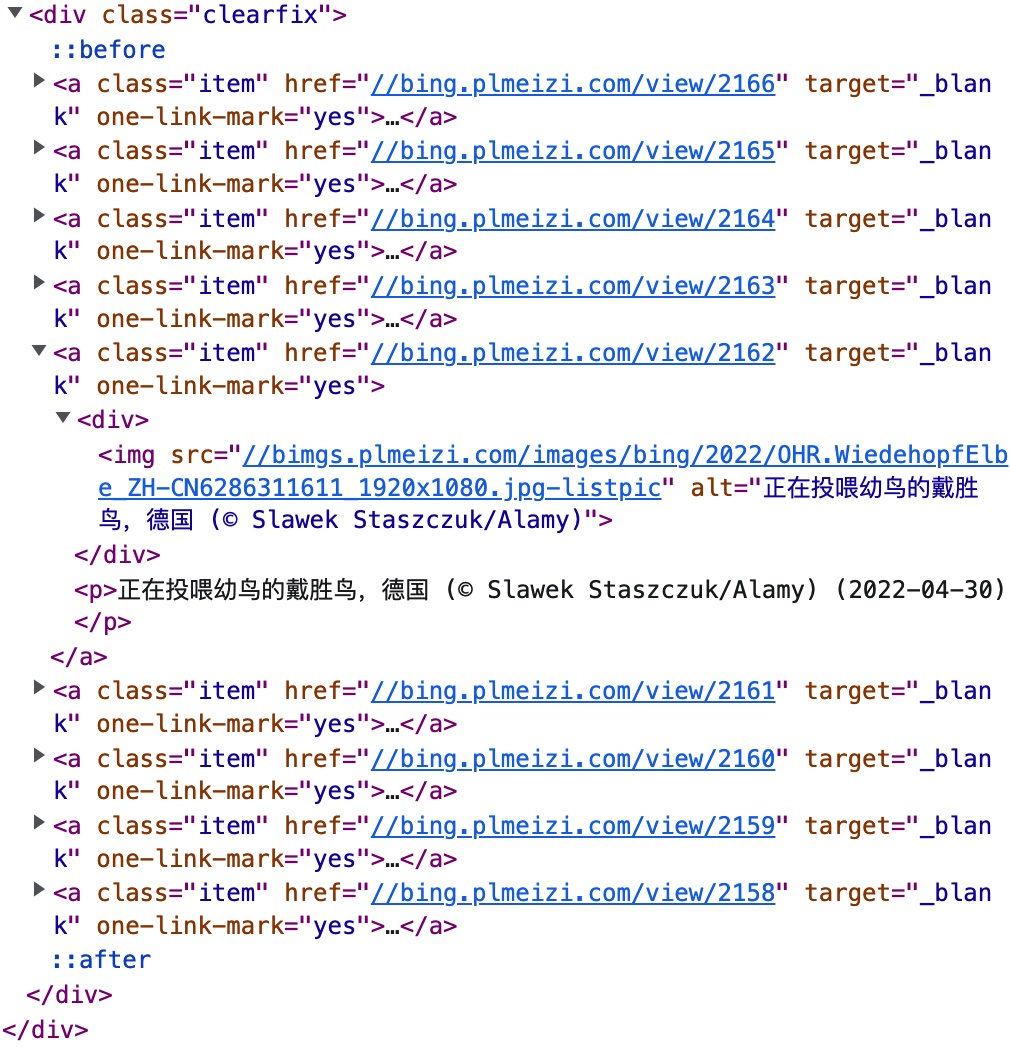
\includegraphics[width=0.6\textwidth]{./images/l3-p4.jpg}
    \caption{部分html代码\label{fig:p4}}
\end{figure}

可以观察到,可以用\mintinline{html}{class="item"}区分出一个图片块,\mintinline{html}{img}块中给出了图片的预览链接,去除链接末尾的\mintinline{text}{-listpic}后缀就理应可以访问到原图。

直接使用\mintinline{text}{wget}下载图片会报403错误,加上http://bing.plmeizi.com/的referer就可以正常下载了。

\paragraph{编写代码}

主体部分是先用\mintinline{text}{sed}和\mintinline{text}{grep}命令划分出我们关心的行,再用\mintinline{text}{sed}命令筛选出有用的信息,存入txt文件中。

下载时从txt文件中依次读取每一行,通过开启后台子进程的方式并行下载。

\begin{code}
\begin{minted}{shell}
#!/bin/bash

if [ $# = 0 ]
then
    from_page=1
    to_page=235
elif [ $# = 2 ]
then
    from_page=$1
    to_page=$2
else
    echo "Usage: $0 <from_page> <to_page>"
    exit 1
fi

if [ ! -d html ]
then
    mkdir html
fi

if [ ! -d temp ]
then
    mkdir temp
fi

if [ ! -d bing ]
then
    mkdir bing
fi

for i in `seq $from_page $to_page`
do
    if [ ! -f html/$i.html ]
    then
        echo -e "\033[33m Downloading... \033[0m html/$i.html"
        wget --no-verbose http://bing.plmeizi.com/?page=$i -O html/$i.html
        echo -e "\033[32m Finished! \033[0m html/$i.html"
    else
        echo -e "\033[34m Existed! \033[0m html/$i.html"
    fi

    if [ ! -f temp/$i.txt ]
    then
        echo -e "\033[33m Downloading... \033[0m temp/$i.txt"
        cat html/$i.html | \
        sed 's/\(<a class="item\)/\n\1/g' | \
        grep 'class="item"' | \
        sed 's#^.*<img src=\(//.*\.jpg\)-listpic .*<p>\(.*\) (.*) (\([0-9]\{4\}-[0-9]\{2\}-[0-9]\{2\}\)).*#http:\1$\2$\3#g' > temp/$i.txt
        echo -e "\033[32m Finished! \033[0m temp/$i.txt"
    else
        echo -e "\033[34m Existed! \033[0m temp/$i.txt"
    fi

    while read line
    do
    {
        url=`echo "$line" | sed 's/\(.*\)$.*$.*/\1/g'`
        img=`echo "$line" | sed 's#.*$\(.*\)$\(.*\)#bing/\2 \1.jpg#g'`
        if [ ! -f "$img" ]
        then
            tmp="$img.downloading$!"
            echo -e "\033[33m Downloading... \033[0m $tmp"
            wget --no-verbose --referer="http://bing.plmeizi.com/" -O "$tmp" $url
            if [ ! $? = 0 ]
            then
                echo -e "\033[31m Failed! \033[0m $tmp"
                rm "$tmp"
                continue
            fi

            if [ ! -f "$img" ]
            then
                echo -e "\033[33m Renaming... \033[0m $tmp to $img"
                mv "$tmp" "$img"
            else
                echo -e "\033[34m Existed! \033[0m $img"
                rm "$tmp"
            fi
            echo -e "\033[32m Finished! \033[0m $img"
        else
            echo -e "\033[34m Existed! \033[0m $img"
        fi
    }&
    done < temp/$i.txt
    wait
done
\end{minted}
\end{code}

\paragraph{运行结果}

运行结果如\figref{fig:p5}。

\begin{figure}[!htb]
    \centering
    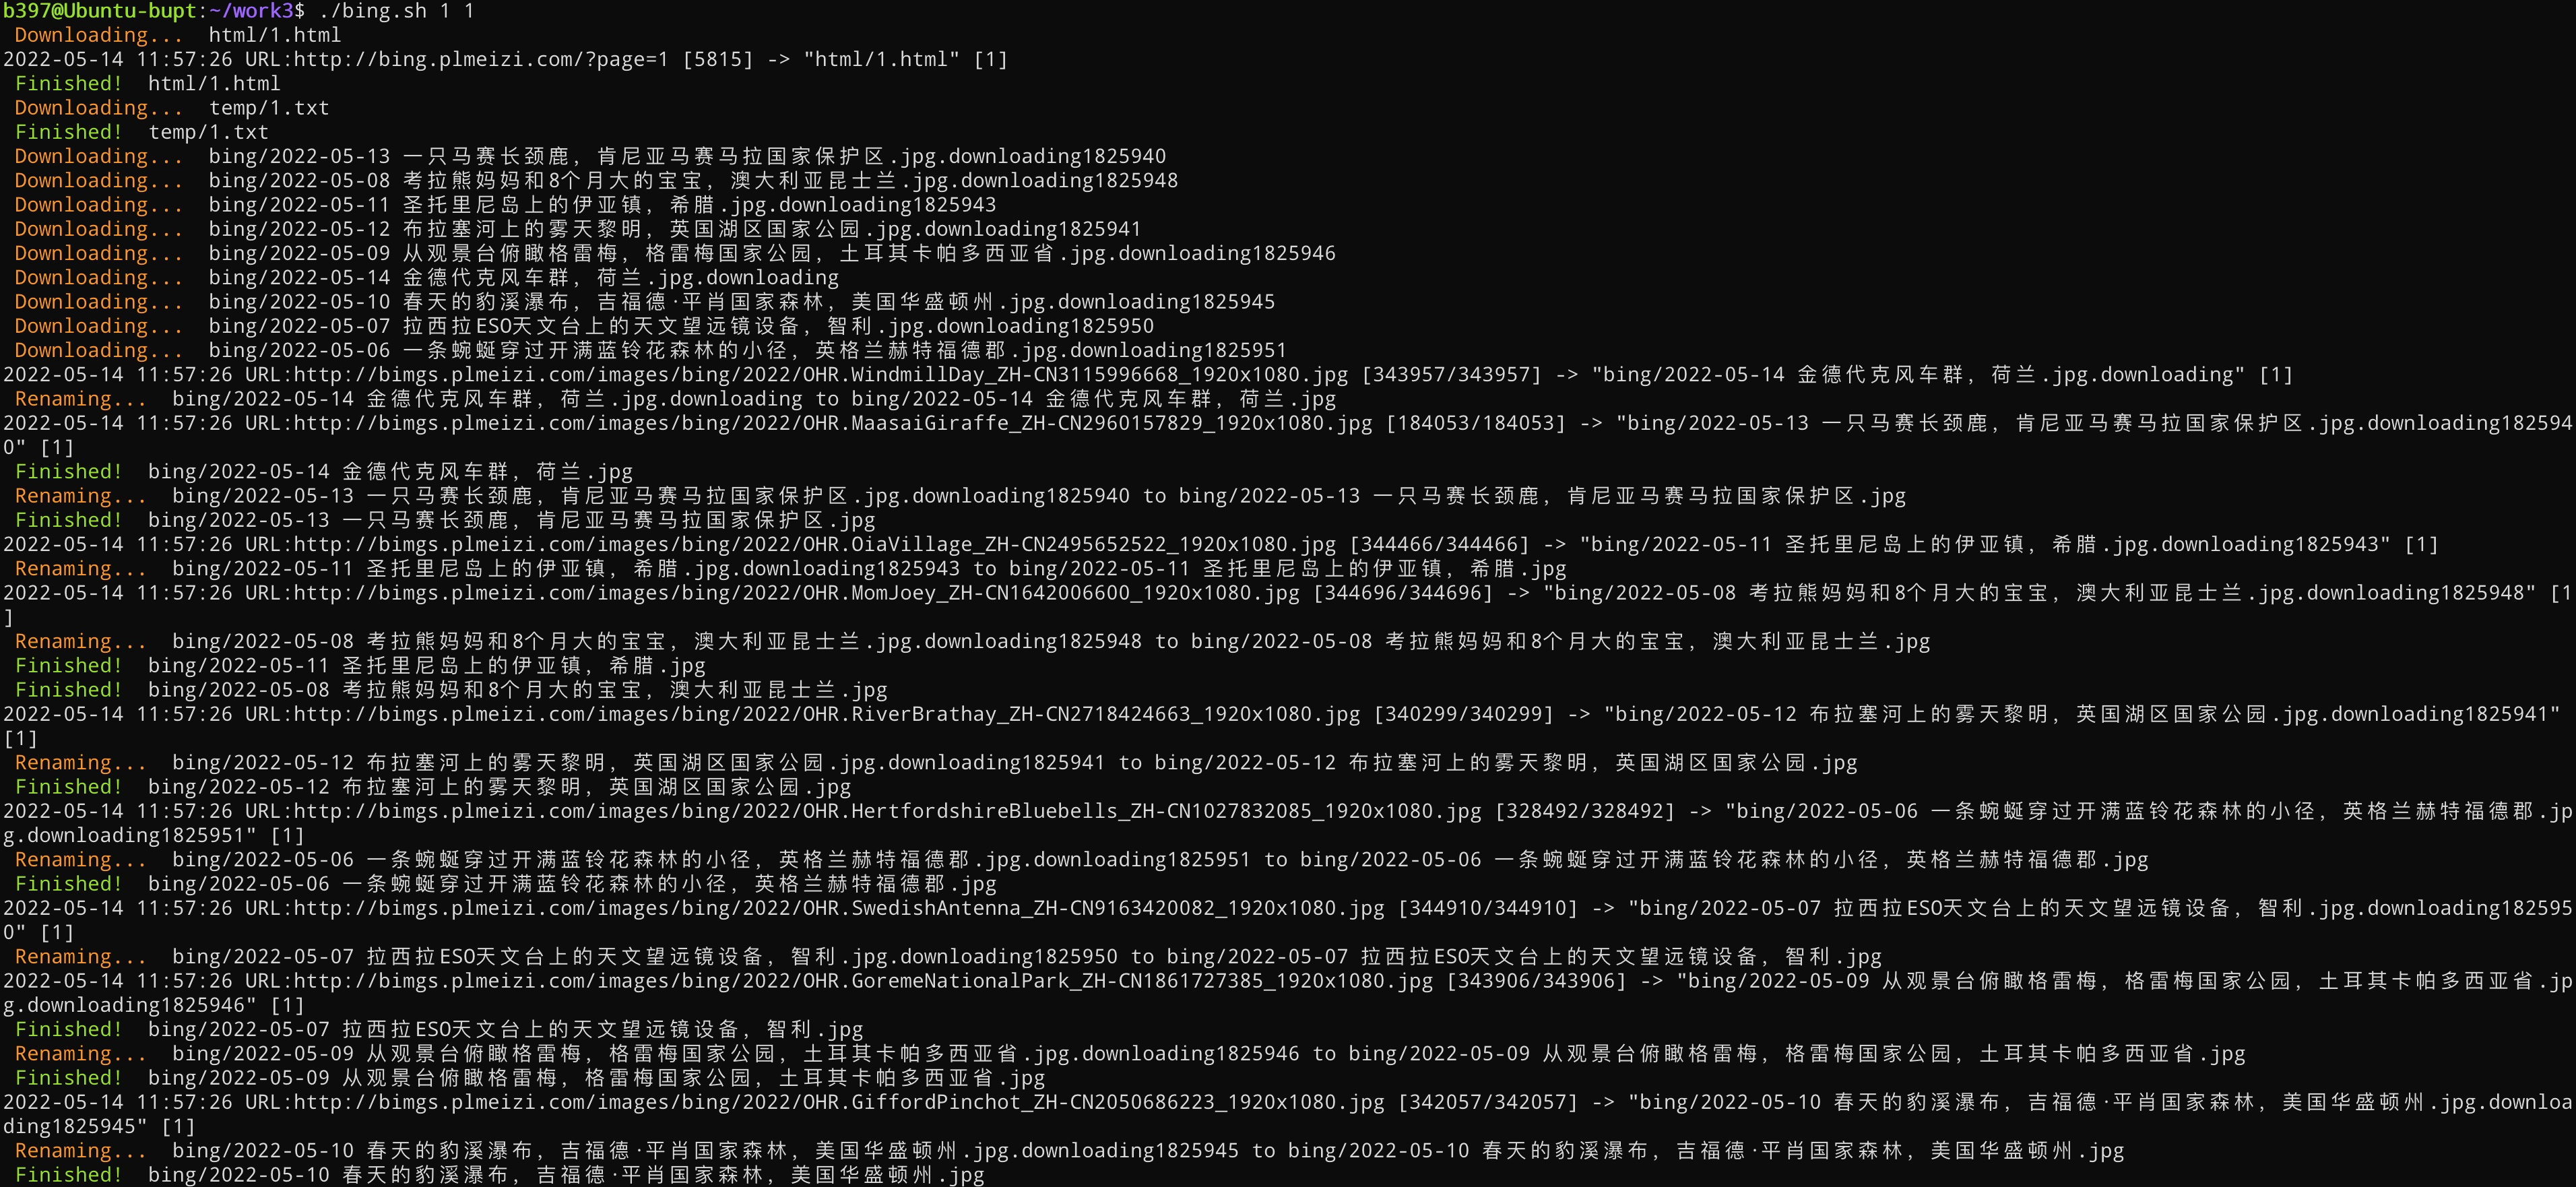
\includegraphics[width=\textwidth]{./images/l3-p5.jpg}

    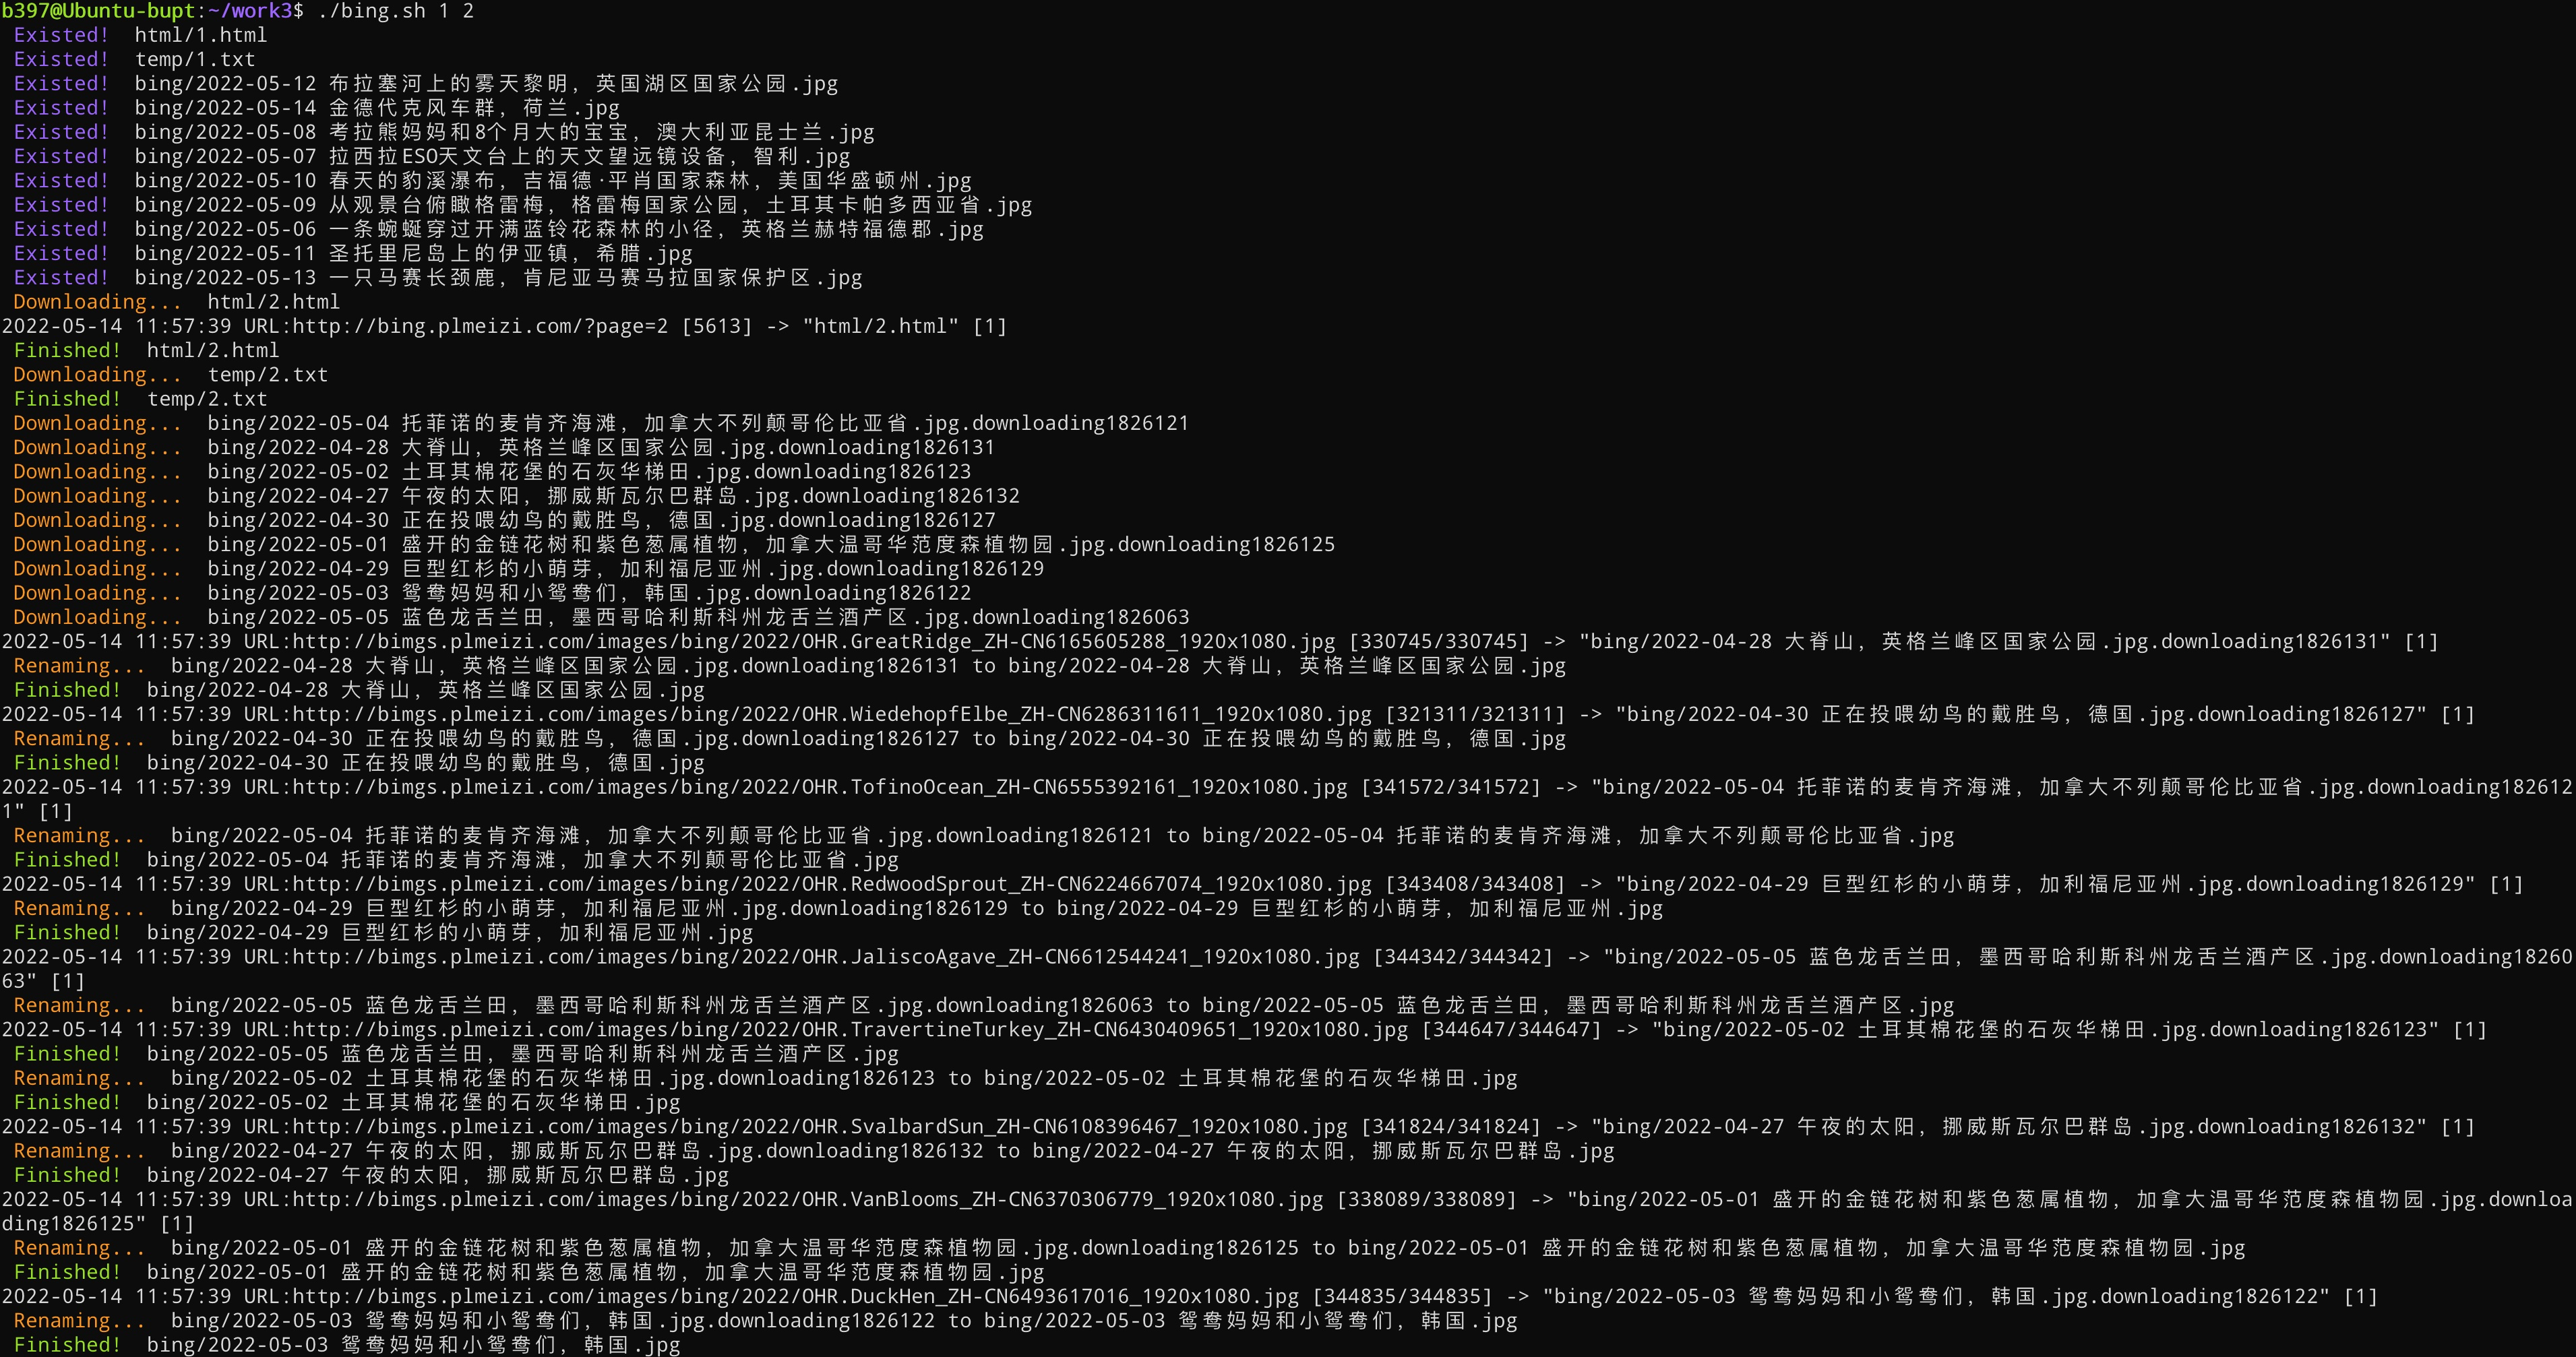
\includegraphics[width=\textwidth]{./images/l3-p6.jpg}

    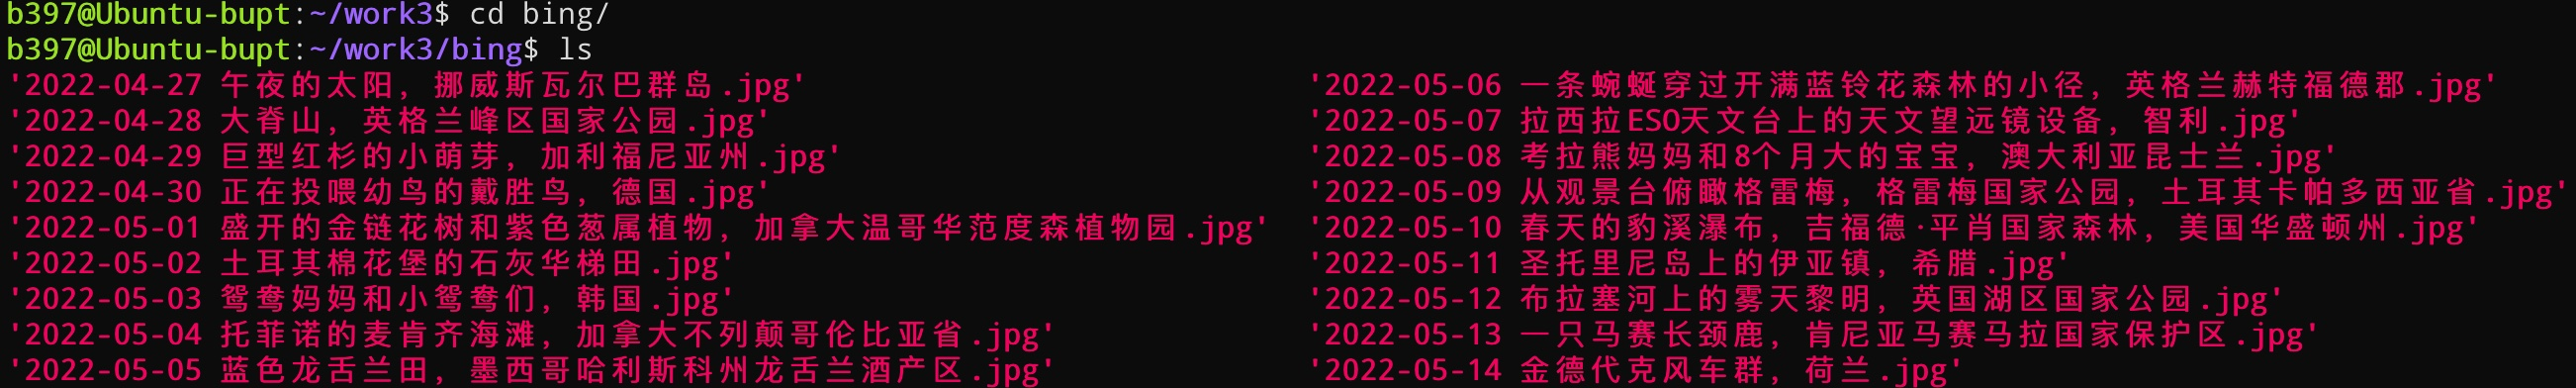
\includegraphics[width=\textwidth]{./images/l3-p7.jpg}
    \caption{运行结果\label{fig:p5}}
\end{figure}

\section{实验总结}

本次实验中我主要应用了\mintinline{text}{expr,echo,sed,grep}等shell指令和\mintinline{text}{if,for,while}编写shell脚本,使我对shell文本编辑和脚本编写更加熟悉。

\end{document}